\section{Bar Graph \cite{wiki-bar-chart}}\label{graph_bar}
A bar chart or bar graph is a chart or graph that presents categorical data with rectangular bars with heights or lengths proportional to the values that they represent. The bars can be plotted vertically or horizontally. A vertical bar chart is sometimes called a \textbf{column chart}\indexlabel{column chart}.


\begin{center}
    \begin{figure}[H]
        \centering
        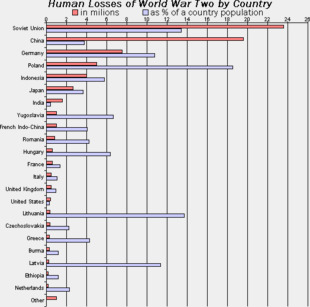
\includegraphics[height=5.6cm]{Pictures/data/data_graph_bar.jpg}
        \caption{Graph: Bar Graph}
    \end{figure}
\end{center}
